\section{Transaction}
\subsection{Mô hình ACID trong MySQL và Redis}

ACID (Atomicity, Consistency, Isolation, Durability) là tập hợp bốn thuộc tính cốt lõi đảm bảo tính đúng đắn và toàn vẹn của transaction trong hệ quản trị cơ sở dữ liệu. Một hệ thống được coi là tuân thủ ACID khi đảm bảo đầy đủ cả bốn tính chất này trong mọi tình huống, kể cả khi xảy ra lỗi hoặc sự cố hệ thống.

\subsubsection{Atomicity (Tính nguyên tử)}

Atomicity đảm bảo rằng một transaction được thực thi như một đơn vị không thể chia nhỏ: hoặc toàn bộ các thao tác được thực hiện thành công, hoặc không có thao tác nào được áp dụng.

Trong MySQL, engine InnoDB cung cấp cơ chế \texttt{COMMIT} và \texttt{ROLLBACK} để đảm bảo tính nguyên tử. Các thay đổi trong transaction được ghi nhận thông qua undo log, cho phép hệ thống hoàn tác toàn bộ khi xảy ra lỗi. Theo tài liệu chính thức, InnoDB hỗ trợ transaction với khả năng commit, rollback và phục hồi sau crash nhằm bảo vệ dữ liệu người dùng .

Ngược lại, Redis cung cấp cơ chế transaction thông qua \texttt{MULTI} và \texttt{EXEC}. Redis đảm bảo rằng các lệnh trong transaction được thực thi tuần tự và không bị xen kẽ bởi các client khác. Tuy nhiên, Redis không hỗ trợ rollback; nếu một lệnh trong transaction thất bại, các lệnh trước đó vẫn giữ nguyên. Điều này cho thấy Redis chỉ đảm bảo atomicity ở mức thực thi tuần tự, không phải atomicity theo nghĩa ACID đầy đủ .

\subsubsection{Consistency (Tính nhất quán)}

Consistency đảm bảo rằng trạng thái của hệ thống luôn chuyển từ một trạng thái hợp lệ sang một trạng thái hợp lệ khác sau khi transaction hoàn tất.

MySQL đảm bảo consistency thông qua các ràng buộc dữ liệu như \texttt{FOREIGN KEY}, \texttt{UNIQUE}, và các quy tắc toàn vẹn. Các ràng buộc này được enforced trực tiếp bởi hệ quản trị cơ sở dữ liệu, giúp ngăn chặn dữ liệu không hợp lệ.

Trong khi đó, Redis không cung cấp cơ chế constraint ở mức hệ thống. Việc đảm bảo consistency phụ thuộc hoàn toàn vào logic của application. Điều này làm tăng tính linh hoạt nhưng đồng thời đặt trách nhiệm đảm bảo tính đúng đắn dữ liệu lên phía lập trình viên.

\subsubsection{Isolation (Tính cô lập)}

Isolation đảm bảo rằng các transaction đồng thời không ảnh hưởng lẫn nhau và kết quả thực thi tương đương với việc thực hiện tuần tự.

MySQL hỗ trợ đầy đủ bốn mức isolation theo chuẩn SQL: Read Uncommitted, Read Committed, Repeatable Read và Serializable. Các mức này được triển khai thông qua cơ chế locking và multi-version concurrency control (MVCC), cho phép kiểm soát sự tương tác giữa các transaction.

Redis, do sử dụng mô hình single-threaded, đảm bảo rằng các lệnh được thực thi tuần tự. Theo tài liệu chính thức, trong một transaction Redis, ``các lệnh được tuần tự hóa và thực thi liên tục, không bị gián đoạn bởi client khác''. Điều này giúp Redis tránh được race condition ở mức command, tuy nhiên không cung cấp isolation theo nghĩa transaction đầy đủ.

\subsubsection{Durability (Tính bền vững)}

Durability đảm bảo rằng sau khi một transaction được commit, các thay đổi sẽ được lưu trữ vĩnh viễn, ngay cả khi hệ thống gặp sự cố.

MySQL sử dụng cơ chế Write-Ahead Logging (WAL) và redo log để đảm bảo dữ liệu được ghi xuống disk trước khi commit hoàn tất. Điều này cho phép hệ thống phục hồi trạng thái dữ liệu sau crash.

Redis cung cấp hai cơ chế persistence chính: RDB (snapshot) và AOF (append-only file). Theo tài liệu Redis, khi sử dụng AOF, các transaction được ghi xuống disk như một thao tác duy nhất, tuy nhiên trong trường hợp crash, có thể xảy ra ghi không đầy đủ và cần phục hồi bằng công cụ chuyên dụng. Do đó, durability trong Redis phụ thuộc vào cấu hình và có thể đánh đổi với hiệu năng.
\begin{table}[H]
\centering
\caption{So sánh mô hình ACID giữa MySQL (InnoDB) và Redis}
\begin{tabular}{|l|p{5.5cm}|p{5.5cm}|}
\hline
\textbf{Thuộc tính} & \textbf{MySQL (InnoDB)} & \textbf{Redis} \\
\hline

\textbf{Atomicity} 
& Đảm bảo đầy đủ thông qua \texttt{COMMIT} và \texttt{ROLLBACK}; sử dụng undo log để hoàn tác toàn bộ transaction khi xảy ra lỗi. 
& Chỉ đảm bảo thực thi tuần tự thông qua \texttt{MULTI/EXEC} hoặc Lua script; không hỗ trợ rollback, do đó không đảm bảo atomicity theo nghĩa ACID đầy đủ. \\
\hline

\textbf{Consistency} 
& Được đảm bảo bởi các ràng buộc dữ liệu như \texttt{FOREIGN KEY}, \texttt{UNIQUE} và các quy tắc toàn vẹn, enforced trực tiếp bởi DBMS. 
& Không có cơ chế constraint ở mức hệ thống; tính nhất quán phụ thuộc vào logic của application. \\
\hline

\textbf{Isolation} 
& Hỗ trợ đầy đủ các mức isolation (Read Uncommitted, Read Committed, Repeatable Read, Serializable) thông qua locking và MVCC. 
& Đảm bảo thực thi tuần tự nhờ mô hình single-threaded; không hỗ trợ isolation theo nghĩa transaction đầy đủ. \\
\hline

\textbf{Durability} 
& Đảm bảo thông qua Write-Ahead Logging (WAL) và redo log; dữ liệu được phục hồi sau crash. 
& Phụ thuộc vào cơ chế persistence (RDB hoặc AOF); durability có thể đánh đổi với hiệu năng và không đảm bảo tuyệt đối trong mọi cấu hình. \\
\hline

\end{tabular}
\end{table}
\subsubsection{Đánh giá tổng hợp}

Từ các phân tích trên, có thể thấy rằng MySQL (InnoDB) là một hệ quản trị cơ sở dữ liệu tuân thủ đầy đủ mô hình ACID, với các cơ chế được tích hợp sâu trong hệ thống để đảm bảo tính toàn vẹn dữ liệu.

Ngược lại, Redis không phải là một hệ ACID-compliant theo nghĩa truyền thống. Redis chỉ cung cấp một số đảm bảo như thực thi tuần tự và atomicity ở mức nhóm lệnh, trong khi các yếu tố như rollback và constraint không được hỗ trợ trực tiếp.

Sự khác biệt này phản ánh hai triết lý thiết kế:
\begin{itemize}
\item MySQL: ưu tiên tính toàn vẹn và nhất quán dữ liệu (strong consistency)
\item Redis: ưu tiên hiệu năng và độ trễ thấp (high performance, eventual correctness)
\end{itemize}


\subsection{Hành vi Transaction trong các kịch bản thực tế}
Để đánh giá cụ thể sự khác biệt trong cơ chế transaction giữa MySQL và Redis, chúng tôi tiến hành triển khai một kịch bản thực tế với đầy đủ các bước xử lý nghiệp vụ.

\subsubsection{Kịch bản: Tạo đơn hàng}

Kịch bản bao gồm ba bước chính:
\begin{itemize}
\item Tạo đơn hàng mới
\item Thêm chi tiết đơn hàng
\item Cập nhật tồn kho
\end{itemize}

Yêu cầu hệ thống là đảm bảo tính toàn vẹn: toàn bộ các thao tác phải thành công hoặc bị hủy bỏ hoàn toàn.

\subsubsection{Triển khai trên MySQL}
\textbf{Kịch bản thành công}
\begin{lstlisting}[
    language=SQL,
    basicstyle=\ttfamily\small,
    columns=fullflexible,
    keepspaces=true,
    breaklines=true,
    frame=single,
    backgroundcolor=\color{gray!10},
    numbers=left,
    numberstyle=\tiny
]
START TRANSACTION;

INSERT INTO sales.orders(customer_id, order_status, order_date, required_date, shipped_date, store_id, staff_id)
VALUES(1, 1, '2026-03-02', '2026-03-10', NULL, 1, 1);

SET @new_order_id = LAST_INSERT_ID();

INSERT INTO sales.order_items(order_id, item_id, product_id, quantity, list_price, discount)
VALUES(@new_order_id, 1, 1, 2, 379.99, 0.10);

UPDATE production.stocks 
SET quantity = quantity - 2
WHERE store_id = 1 AND product_id = 1;

COMMIT;
\end{lstlisting}

Dữ liệu trước khi thực thi transaction
\begin{figure}[H]
\centering
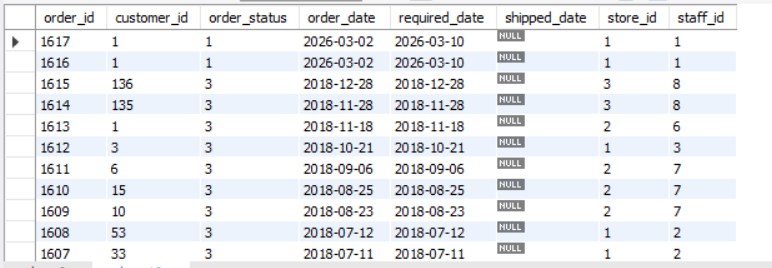
\includegraphics[width=0.9\textwidth]{figures/Thời/order-before-transaction.png}
\caption{Bảng orders trước khi transaction}
\end{figure}

\begin{figure}[H]
\centering
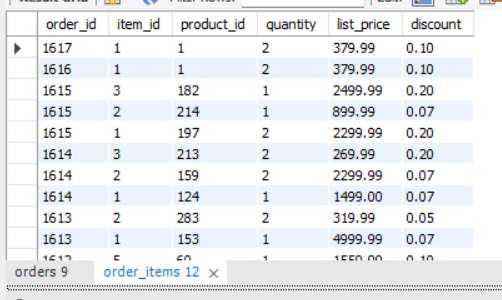
\includegraphics[width=0.9\textwidth]{figures/Thời/item-before-transaction.png}
\caption{Bảng order\_items trước khi transaction}
\end{figure}

\begin{figure}[H]
    \centering
    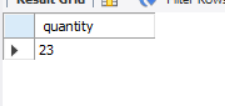
\includegraphics[width=0.7\textwidth]{figures/Thời/stock-before-transaction.png}
    \caption{Bảng stocks có product\_id = 1 và store\_id = 1 trước khi transaction}
\end{figure}

Dữ liệu sau khi thực thi transaction
\begin{figure}[H]
    \centering
    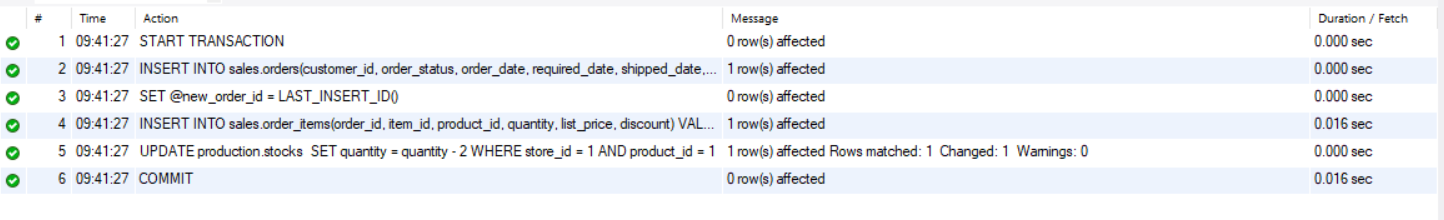
\includegraphics[width=0.9\textwidth]{figures/Thời/after-transaction.png}
    \caption{Thông báo lệnh thực thi thành công}
\end{figure}

\begin{figure}[H]
\centering
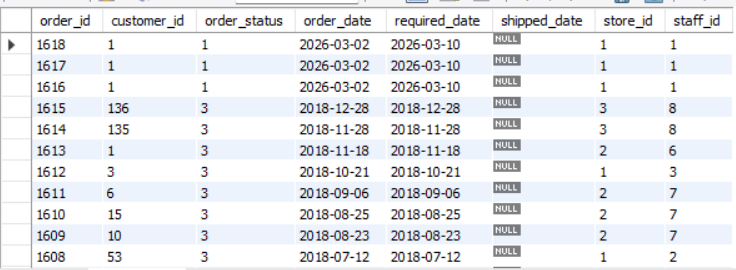
\includegraphics[width=0.9\textwidth]{figures/Thời/order-after-transaction.png}
\caption{Bảng orders sau khi transaction}
\end{figure}

\begin{figure}[H]
\centering
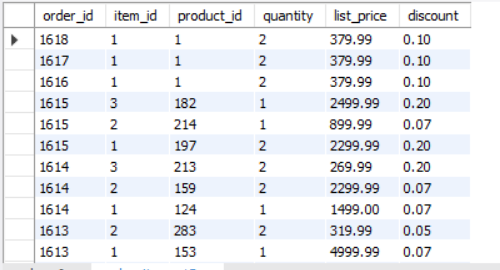
\includegraphics[width=0.9\textwidth]{figures/Thời/item-after-transaction.png}
\caption{Bảng order\_items sau khi transaction}
\end{figure}

\begin{figure}[H]
\centering
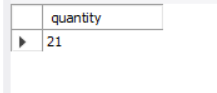
\includegraphics[width=0.7\textwidth]{figures/Thời/stock-after-transaction.png}
\caption{Bảng stocks có product\_id = 1 và store\_id = 1 sau khi transaction}
\end{figure}
\textbf{Phân tích:}

Kết quả thực nghiệm cho thấy transaction đã được thực thi thành công, khi toàn bộ các thao tác bao gồm thêm bản ghi vào bảng \texttt{orders}, thêm dữ liệu vào bảng \texttt{order\_items} và cập nhật tồn kho trong bảng \texttt{stocks} đều được áp dụng.

Cụ thể, bản ghi mới xuất hiện trong bảng \texttt{orders} với \texttt{order\_id} tương ứng, đồng thời các bản ghi liên quan trong bảng \texttt{order\_items} cũng được tạo ra với khóa ngoại trỏ về đơn hàng này. Bên cạnh đó, giá trị tồn kho trong bảng \texttt{production.stocks} đã giảm đúng theo số lượng đặt hàng, phản ánh việc cập nhật dữ liệu được thực hiện chính xác.

Kết quả này chứng minh rằng MySQL đảm bảo tính \textbf{Atomicity}, khi toàn bộ các thao tác trong transaction được thực hiện như một đơn vị duy nhất và chỉ được ghi nhận khi tất cả đều thành công. Không tồn tại trạng thái trung gian trong đó chỉ một phần dữ liệu được cập nhật.

Ngoài ra, tính \textbf{Consistency} cũng được duy trì, khi các ràng buộc khóa ngoại giữa các bảng (\texttt{orders}, \texttt{order\_items}, \texttt{products}, \texttt{stocks}) vẫn được đảm bảo. Điều này cho thấy dữ liệu sau transaction vẫn nằm trong trạng thái hợp lệ theo các quy tắc toàn vẹn đã định nghĩa.

Bên cạnh đó, cơ chế transaction của InnoDB còn đảm bảo \textbf{Isolation}, khi các thao tác được thực thi mà không bị ảnh hưởng bởi các transaction đồng thời, và \textbf{Durability}, khi các thay đổi được ghi nhận vĩnh viễn sau khi \texttt{COMMIT}.

\textbf{Nhận xét:}

Kịch bản này minh họa rõ ràng cách MySQL thực thi transaction theo mô hình ACID, trong đó database đóng vai trò trung tâm trong việc đảm bảo tính toàn vẹn và nhất quán dữ liệu, mà không yêu cầu logic xử lý phức tạp từ phía application.

\textbf{Kịch bản thất bại (Rollback)}


\textbf{Mô tả:}

Trong kịch bản này, transaction được thực hiện với điều kiện tồn kho không đủ để đáp ứng số lượng đặt hàng. Khi thao tác cập nhật tồn kho dẫn đến giá trị âm, transaction được kỳ vọng sẽ bị hủy bỏ nhằm đảm bảo tính toàn vẹn dữ liệu.

\textbf{Thực thi:}

\begin{lstlisting}[
    language=SQL,
    basicstyle=\ttfamily\small,
    columns=fullflexible,
    keepspaces=true,
    breaklines=true,
    frame=single,
    backgroundcolor=\color{gray!10},
    numbers=left,
    numberstyle=\tiny
]
DELIMITER //

CREATE PROCEDURE test_tx()
BEGIN
    DECLARE v_stock INT;

    START TRANSACTION;

    UPDATE production.stocks 
    SET quantity = quantity - 5
    WHERE store_id = 1 AND product_id = 6;

    SELECT quantity INTO v_stock
    FROM production.stocks 
    WHERE store_id = 1 AND product_id = 6;

    IF v_stock < 0 THEN
        ROLLBACK;
    ELSE
        COMMIT;
    END IF;

END //

DELIMITER ;
CALL test_tx();

\end{lstlisting}

Dữ liệu trước khi thực thi:
\begin{figure}[H]
\centering
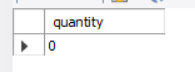
\includegraphics[width=0.7\textwidth]{figures/Thời/stock-before-rollback.png}
\caption{Bảng stocks có product\_id = 6 và store\_id = 1 trước khi transaction}
\end{figure}

Dữ liệu sau khi thực thi:
\begin{figure}[H]
\centering
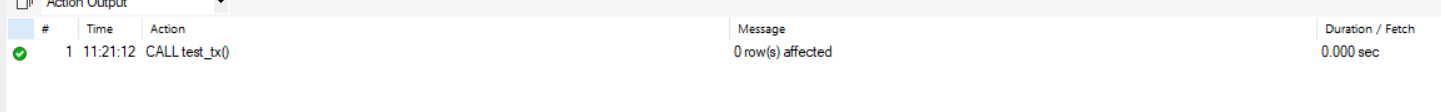
\includegraphics[width=0.9\textwidth]{figures/Thời/after-excute-rollback.png}
\caption{Kết quả sau khi thực thi procedure test\_tx}
\end{figure}

\begin{figure}[H]
\centering
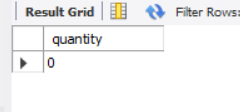
\includegraphics[width=0.7\textwidth]{figures/Thời/stock-after-rollback.png}
\caption{Bảng stocks có product\_id = 6và store\_id = 1 sau khi transaction}
\end{figure}

\textbf{Phân tích:}

Kết quả thực nghiệm cho thấy khi một điều kiện không hợp lệ xảy ra trong transaction (cụ thể là tồn kho không đủ), toàn bộ transaction đã bị rollback. Điều này đảm bảo rằng không có bất kỳ thay đổi nào được ghi nhận trong hệ thống, kể cả những thao tác đã thực hiện trước đó trong transaction.

Cơ chế này phản ánh rõ tính \textbf{Atomicity}, khi transaction được xem như một đơn vị không thể chia nhỏ: hoặc tất cả các thao tác đều thành công, hoặc không có thao tác nào được áp dụng. Trong trường hợp này, việc cập nhật tồn kho không hợp lệ đã khiến toàn bộ transaction bị hủy bỏ.

Ngoài ra, tính \textbf{Consistency} cũng được đảm bảo, khi hệ thống không rơi vào trạng thái dữ liệu không hợp lệ (ví dụ tồn kho âm hoặc tồn tại order không hợp lệ). Các ràng buộc toàn vẹn dữ liệu vẫn được duy trì sau khi rollback.

Cơ chế rollback của InnoDB dựa trên undo log, cho phép khôi phục trạng thái dữ liệu trước khi transaction bắt đầu. Điều này đặc biệt quan trọng trong các hệ thống thực tế, nơi các thao tác thường phụ thuộc lẫn nhau và cần được thực hiện một cách toàn vẹn.

\textbf{Nhận xét:}

Kịch bản thất bại minh họa vai trò quan trọng của transaction trong việc bảo vệ dữ liệu khỏi các trạng thái không nhất quán. Khả năng rollback là một trong những yếu tố cốt lõi giúp MySQL tuân thủ đầy đủ mô hình ACID, đặc biệt trong các nghiệp vụ phức tạp như quản lý đơn hàng và tồn kho.

\subsubsection{Triển khai trên Redis}
\textbf{Kịch bản thành công}
\begin{lstlisting}[
    language=SQL,
    basicstyle=\ttfamily\small,
    columns=fullflexible,
    keepspaces=true,
    breaklines=true,
    frame=single,
    backgroundcolor=\color{gray!10},
    numbers=left,
    numberstyle=\tiny
]
MULTI
INCR sales:orders:next_id
HSET sales:order:1616 customer_id 1 order_status 1 order_date "2026-03-02" required_date "2026-03-10" shipped_date "" store_id 1 staff_id 1
SADD sales:orders:ids 1616
SADD sales:orders:customer:1 1616
SADD sales:orders:store:1 1616
HSET sales:order_item:1616:1 product_id 1 quantity 2 list_price 379.99 discount 0.10
SADD sales:order_items:order:1616 1
HINCRBY production:stock:1:1 quantity -2
EXEC
\end{lstlisting}

Trước khi thực thi:
Trong bộ dữ liệu được cung cấp, order có 1615 rows. Vì vậy order\_id 1616 chưa tồn tại trong hệ thống.
\begin{figure}[H]
\centering
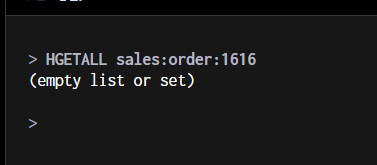
\includegraphics[width=0.7\textwidth]{figures/Thời/redis-order-before-success.png}
\caption{Kết quả tìm kiếm order có id 1616}
\end{figure}

\begin{figure}[H]
\centering
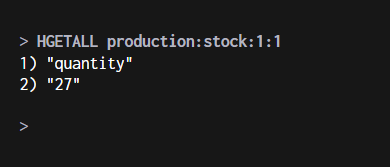
\includegraphics[width=0.7\textwidth]{figures/Thời/redis-stock-before-success.png}
\caption{Kết quẩ tìm kiếm stock có product\_id = 1 và store\_id = 1 trong redis trước khi thực thi transaction}
\end{figure}

Sau khi thực thi:
\begin{figure}[H]
\centering
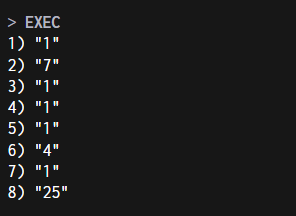
\includegraphics[width=0.7\textwidth]{figures/Thời/redis-after-excute.png}
\caption{Sau khi chạy tổ hợp các câu lệnh trên}
\end{figure}

\begin{figure}[H]
\centering
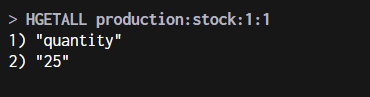
\includegraphics[width=0.7\textwidth]{figures/Thời/redis-stock-after-success.png}
\caption{Kết quẩ tìm kiếm stock có product\_id = 1 và store\_id = 1 trong redis sau khi thực thi thành công}
\end{figure}

\begin{figure}[H]
\centering
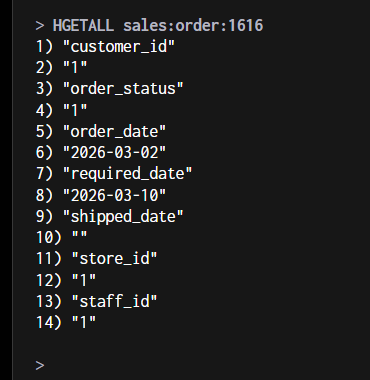
\includegraphics[width=0.7\textwidth]{figures/Thời/redis-order-after-success.png}
\caption{Kết quẩ tìm kiếm order có id = 1616 sau khi thực thi thành công}
\end{figure}

Bên cạnh đó, ta có thể dùng Lua script để gom hết các lệnh vào 1 block nguyên tử
% Hoặc sử dụng Lua script:
\begin{lstlisting}[
    language=SQL,
    basicstyle=\ttfamily\small,
    columns=fullflexible,
    keepspaces=true,
    breaklines=true,
    frame=single,
    backgroundcolor=\color{gray!10},
    numbers=left,
    numberstyle=\tiny,
    showspaces=false,
    showstringspaces=false
]
EVAL "
local oid = 1617
redis.call('HSET', 'sales:order:' .. oid,
    'customer_id', '1', 'order_status', '1',
    'order_date', '2026-03-02', 'required_date', '2026-03-10',
    'shipped_date', '', 'store_id', '1', 'staff_id', '1')
redis.call('SADD', 'sales:orders:ids', oid)
redis.call('HINCRBY', 'production:stock:1:1', 'quantity', -2)
return 'OK'
" 0
\end{lstlisting}

\begin{figure}[H]
\centering
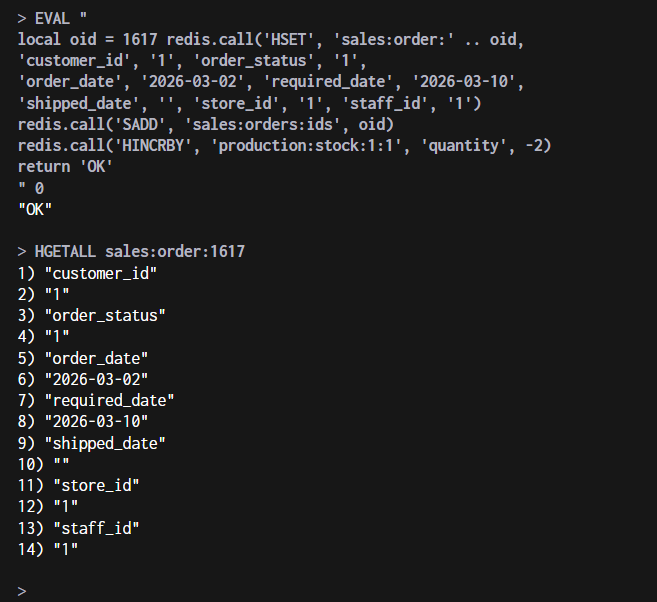
\includegraphics[width=0.7\textwidth]{figures/Thời/redis-lua-success.png}
\caption{Kết quả sau khi thực thi Lua script thành công}
\end{figure}

\textbf{Kịch bản thất bại}
\begin{lstlisting}[
    language=SQL,
    basicstyle=\ttfamily\small,
    columns=fullflexible,
    keepspaces=true,
    breaklines=true,
    frame=single,
    backgroundcolor=\color{gray!10},
    numbers=left,
    numberstyle=\tiny,
    showspaces=false,
    showstringspaces=false
]
EVAL "
local stock = tonumber(redis.call('HGET', 'production:stock:1:6', 'quantity'))
if stock < 5 then
    return 'FAILED: Not enough stock (have ' .. stock .. ', need 5)'
end
redis.call('HINCRBY', 'production:stock:1:6', 'quantity', -5)
return 'OK: Stock reduced to ' .. (stock - 5)
" 0
\end{lstlisting}
\begin{figure}[H]
\centering
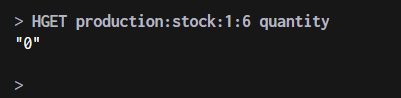
\includegraphics[width=0.7\textwidth]{figures/Thời/redis-stock-before-fail.png}
\caption{Quantity của stock có product\_id = 6 và store\_id = 1 trước khi thực thi}
\end{figure}

\begin{figure}[H]
\centering
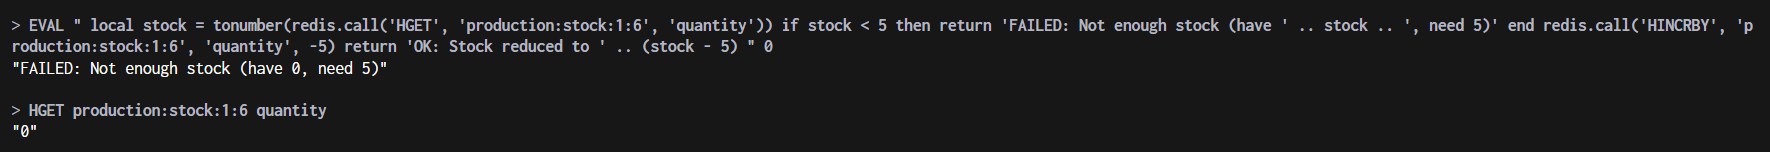
\includegraphics[width=\textwidth]{figures/Thời/redis-stock-after-fail.png}
\caption{Quantity của stock có product\_id = 6 và store\_id = 1 sau khi thực thi}
\end{figure}
\textbf{Phân tích:}

Redis đảm bảo rằng các lệnh trong khối \texttt{MULTI/EXEC} được thực thi tuần tự và không bị xen kẽ bởi các client khác, từ đó duy trì tính nhất quán trong quá trình thực thi. Tuy nhiên, cơ chế này không cung cấp khả năng rollback. Khi xảy ra lỗi logic hoặc điều kiện không hợp lệ, các lệnh đã được thực thi vẫn không thể bị hoàn tác, dẫn đến nguy cơ dữ liệu bị thay đổi không mong muốn.

Việc sử dụng Lua script cho phép đóng gói toàn bộ logic kiểm tra và cập nhật trong một khối thực thi nguyên tử duy nhất. Điều này giúp ngăn chặn các thay đổi không hợp lệ bằng cách dừng thực thi trước khi dữ liệu bị sửa đổi. Tuy nhiên, cách tiếp cận này mang tính chất \textit{phòng ngừa} (preventive) hơn là \textit{khôi phục} (recovery), và do đó không thể thay thế hoàn toàn cơ chế transaction với rollback như trong MySQL.

\textbf{Cơ chế WATCH (Optimistic Locking) trong Redis} \\

Redis cung cấp lệnh \texttt{WATCH} như một cơ chế \textit{optimistic locking} để phát hiện xung đột khi nhiều client cùng thao tác trên một key. Khi một key được theo dõi, Redis sẽ kiểm tra xem key đó có bị thay đổi trước khi \texttt{EXEC} được gọi hay không.

Nếu key bị thay đổi bởi client khác, toàn bộ transaction sẽ bị hủy và \texttt{EXEC} trả về \texttt{nil}; ngược lại, các lệnh sẽ được thực thi bình thường. Cơ chế này giúp ngăn chặn việc cập nhật dữ liệu không nhất quán, tuy nhiên không cung cấp khả năng rollback như trong MySQL.

Để minh họa cơ chế phát hiện xung đột này, đoạn mã dưới đây mô phỏng hai client truy cập đồng thời vào cùng một key:

\begin{lstlisting}[
    language=SQL,
    basicstyle=\ttfamily\small,
    columns=fullflexible,
    keepspaces=true,
    breaklines=true,
    frame=single,
    backgroundcolor=\color{gray!10},
    numbers=left,
    numberstyle=\tiny
]
-- Terminal 1
redis-cli WATCH production:stock:1:1
redis-cli MULTI
redis-cli HINCRBY production:stock:1:1 quantity -1

-- Terminal 2:
redis-cli HSET production:stock:1:1 quantity 100

-- Terminal 1
redis-cli EXEC
\end{lstlisting}

\begin{figure}[H]
\centering
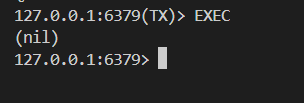
\includegraphics[width=\textwidth]{figures/Thời/redis-watch.png}
\caption{Kết quả sau khi thực thi các câu lệnh trên}
\end{figure}

\subsection{Nhận xét so sánh}

\begin{itemize}
\item MySQL đảm bảo transaction ở mức hệ quản trị cơ sở dữ liệu, với đầy đủ các thuộc tính ACID, đặc biệt là khả năng rollback nhằm khôi phục trạng thái dữ liệu khi xảy ra lỗi.
\item Redis chỉ đảm bảo tính nguyên tử (atomicity) ở mức thực thi lệnh hoặc khối lệnh (thông qua \texttt{MULTI/EXEC} hoặc Lua script), nhưng không hỗ trợ cơ chế rollback khi xảy ra sai sót logic.
\item Trong Redis, trách nhiệm đảm bảo tính đúng đắn và nhất quán của dữ liệu được chuyển sang tầng ứng dụng hoặc logic xử lý (ví dụ: kiểm tra điều kiện trước khi cập nhật bằng Lua script).
\end{itemize}

\noindent
Nhìn chung, MySQL phù hợp với các hệ thống yêu cầu tính toàn vẹn dữ liệu nghiêm ngặt và cơ chế kiểm soát transaction mạnh mẽ, trong khi Redis ưu tiên hiệu năng và tính đơn giản, chấp nhận đánh đổi bằng việc giảm bớt các cơ chế bảo vệ dữ liệu ở mức hệ quản trị.
